\begin{frame}[fragile,t]
  \frametitle{Taylor-mode Automatic Differentiation (Vector Case)}

  \vspace{0.5ex}
  \uncover<4->{
    \emph{Example:} Laplacian \quad $\Delta f^{(L)}(\vx) = \sum_j \frac{\partial^2 f^{(L)}(\vx)}{\partial x_j^2} = \sum_j \partial^2_{\ve_j} f^{(L)}(\vx)$
  }
  \vspace{0ex}

  \begin{figure}[t]
    \centering
    \hspace*{-3ex}
    \begin{tikzpicture}
      \matrix (magic)
      [matrix of nodes,
      ampersand replacement=\&,
      nodes={
        anchor=center,
        inner sep=2pt,
      }]
      {
        \textcolor{orange}{\textbf{Taylor}}
        \&$f^{(0)} = \operatorname{id}$
        \& $f^{(1)} \circ f^{(0)}$
        \& $\dots$
        \& $f^{(L)} \circ \ldots \circ f^{(0)}$
        \\
        \textcolor{orange}{\textbf{2\textsuperscript{nd}-order}}
        \& 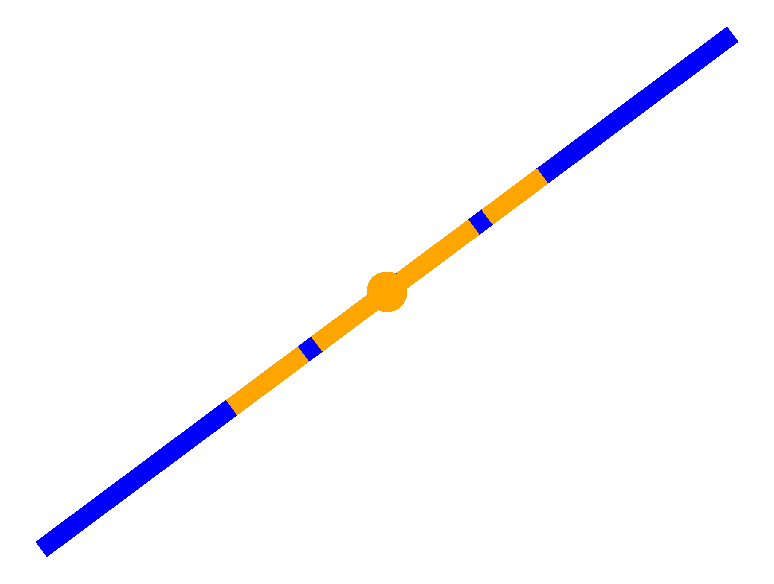
\includegraphics[scale=0.23]{/Users/fdangel/Documents/Postdoc/kfac-pinns/kfac_pinns_exp/exp48_visualization_taylor_mode/f_0_taylor_2.pdf}
        \& 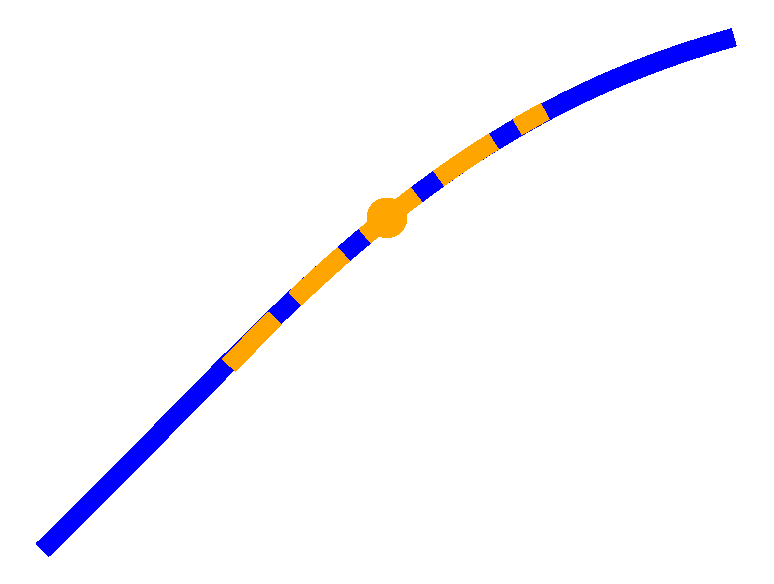
\includegraphics[scale=0.23]{/Users/fdangel/Documents/Postdoc/kfac-pinns/kfac_pinns_exp/exp48_visualization_taylor_mode/f_1_taylor_2.pdf}
        \& 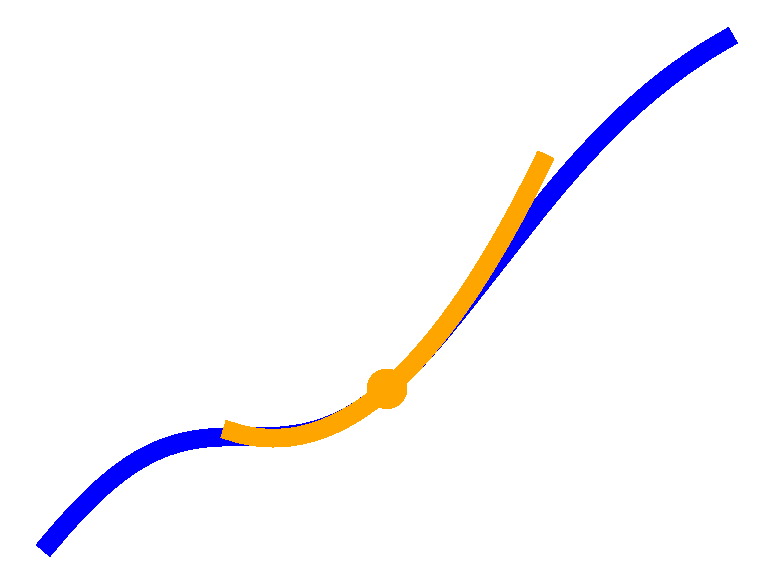
\includegraphics[scale=0.23]{/Users/fdangel/Documents/Postdoc/kfac-pinns/kfac_pinns_exp/exp48_visualization_taylor_mode/f_2_taylor_2.pdf}
        \& 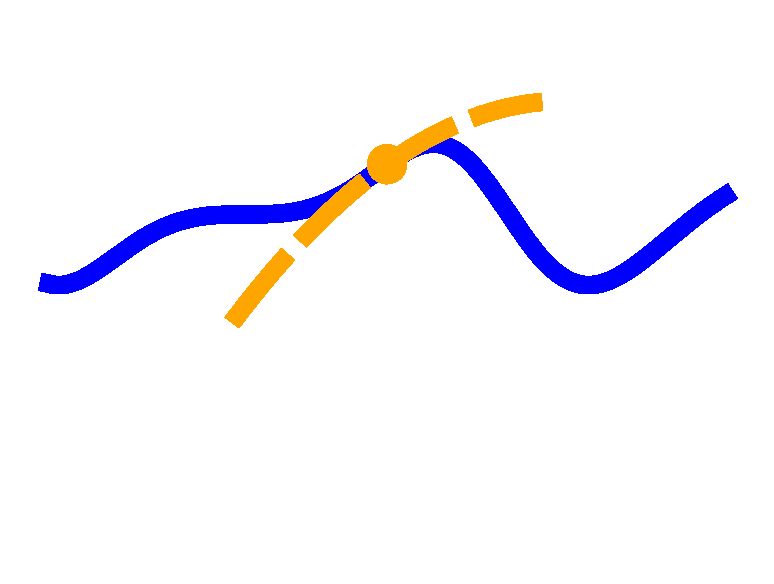
\includegraphics[scale=0.23]{/Users/fdangel/Documents/Postdoc/kfac-pinns/kfac_pinns_exp/exp48_visualization_taylor_mode/f_3_taylor_2.pdf}
        \\
        \& $f^{(0)}(\vx) = \vx$
        \& $\left\{ f_i^{(1)}(f^{(0)}(\vx)) \right\}_i$
        \&$\dots$
        \&$\left\{ f_i^{(L)}(f^{(L-1)}(\vx)) \right\}_i$
        \\
        \only<2->{
          \&$\left\{\partial_{\vv} f_i^{(0)}(\vx) = v_{i}\right\}_i$
          \&$\left\{\partial_{\vv} f_i^{(1)}(\vx) \right\}_i$
          \&$\dots$
          \&$\left\{\partial_{\vv} f_i^{(L)}(\vx) \right\}_i$
        }
        \\
        \only<3->{
          \&$\left\{\partial^2_{\vv} f_i^{(0)}(\vx) = 0 \right\}_i$
          \&$\left\{\partial^2_{\vv} f_i^{(1)}(\vx) \right\}_i$
          \&$\dots$
          \&$\left\{\partial^2_{\vv} f_i^{(L)}(\vx) \right\}_i$
        }
        \\
      };
    \end{tikzpicture}
  \end{figure}
\end{frame}
%%% Local Variables:
%%% mode: LaTeX
%%% TeX-master: "../pitch"
%%% End:
